\begin{frame}{Compress Quadrature}
  \begin{outline}
    \1 Voxel Example
    \1 Show the CT scan photo
  \end{outline}

    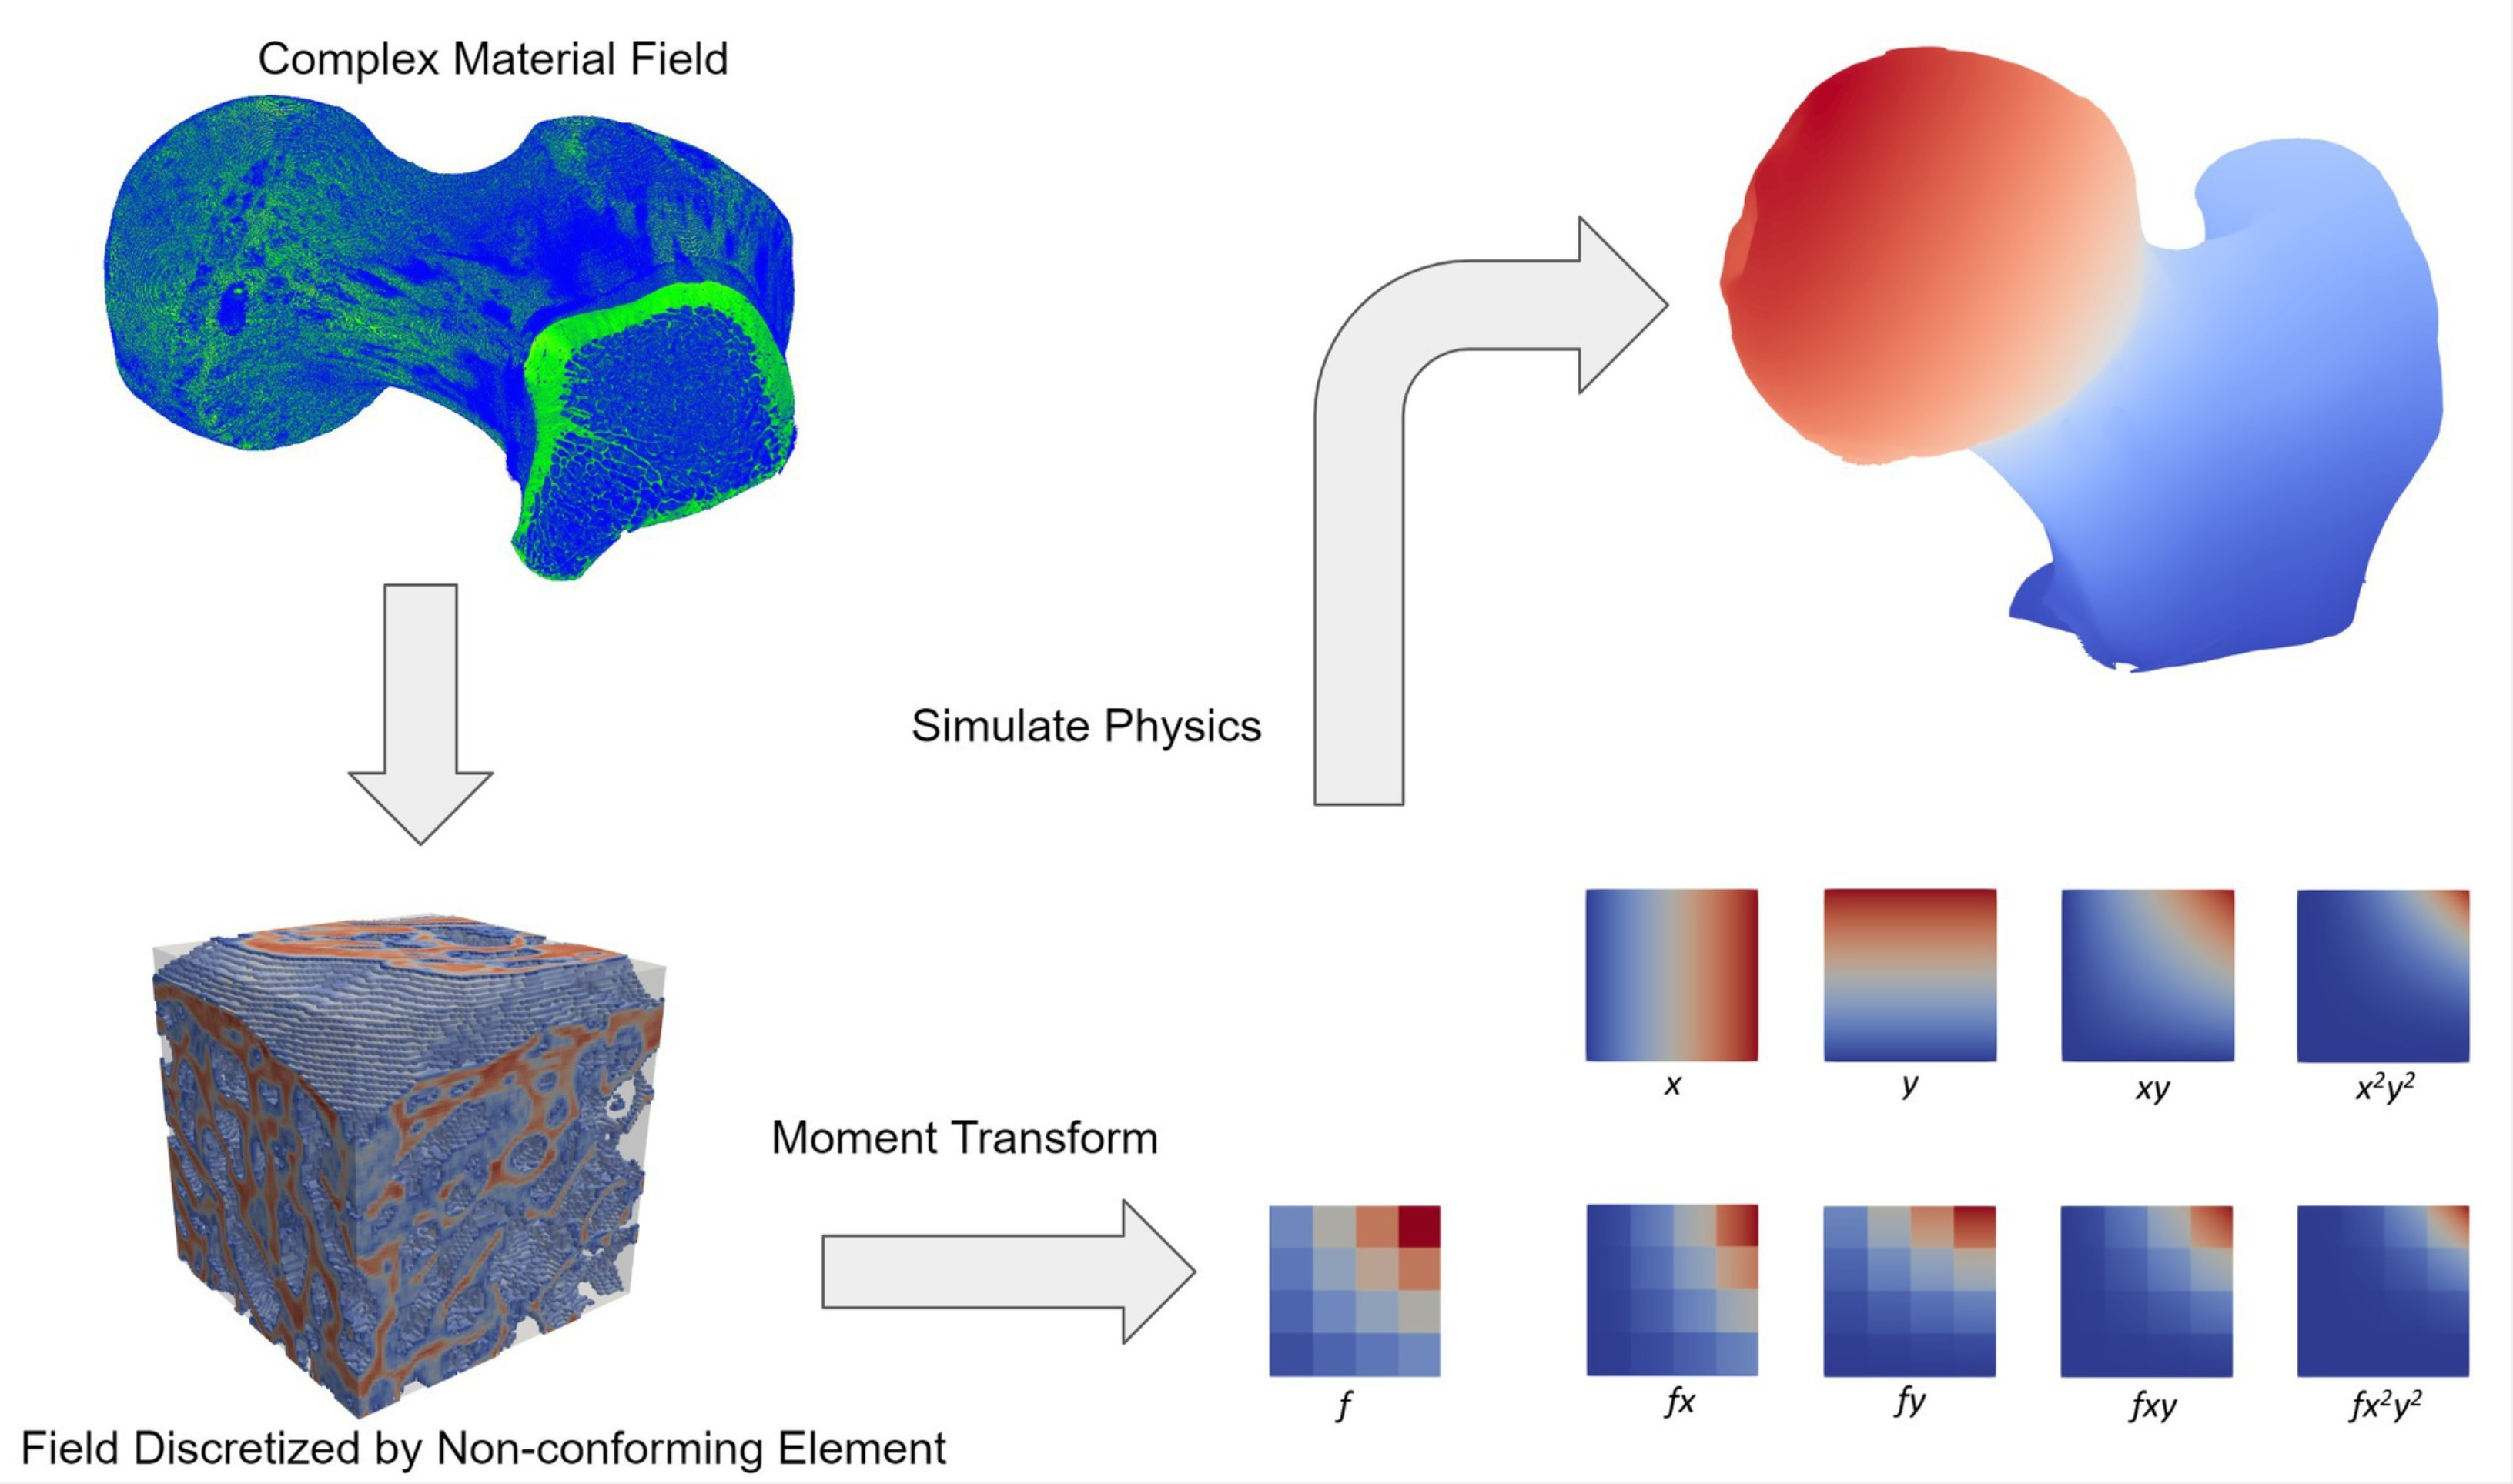
\includegraphics[width=6cm]{bone_scan_example.png}\\

    \blfootnote{Image from \cite{Taber2018}}
\end{frame}

\begin{frame}{Using the Divergence Theorem}
  \begin{outline}
\1 Use divergence theorem to integrate moments over boundary
  \end{outline}
\end{frame}

\begin{frame}{Consequences}
\begin{columns}
\column{0.58\linewidth}
  \begin{outline}
    \1 Generalizes from just density to other fields like conductivity or even stiffness (spatially variable materials)
    \1 This was my job, shuttling data where it needs to be
  \end{outline}
\column{0.38\linewidth}
\begin{center}
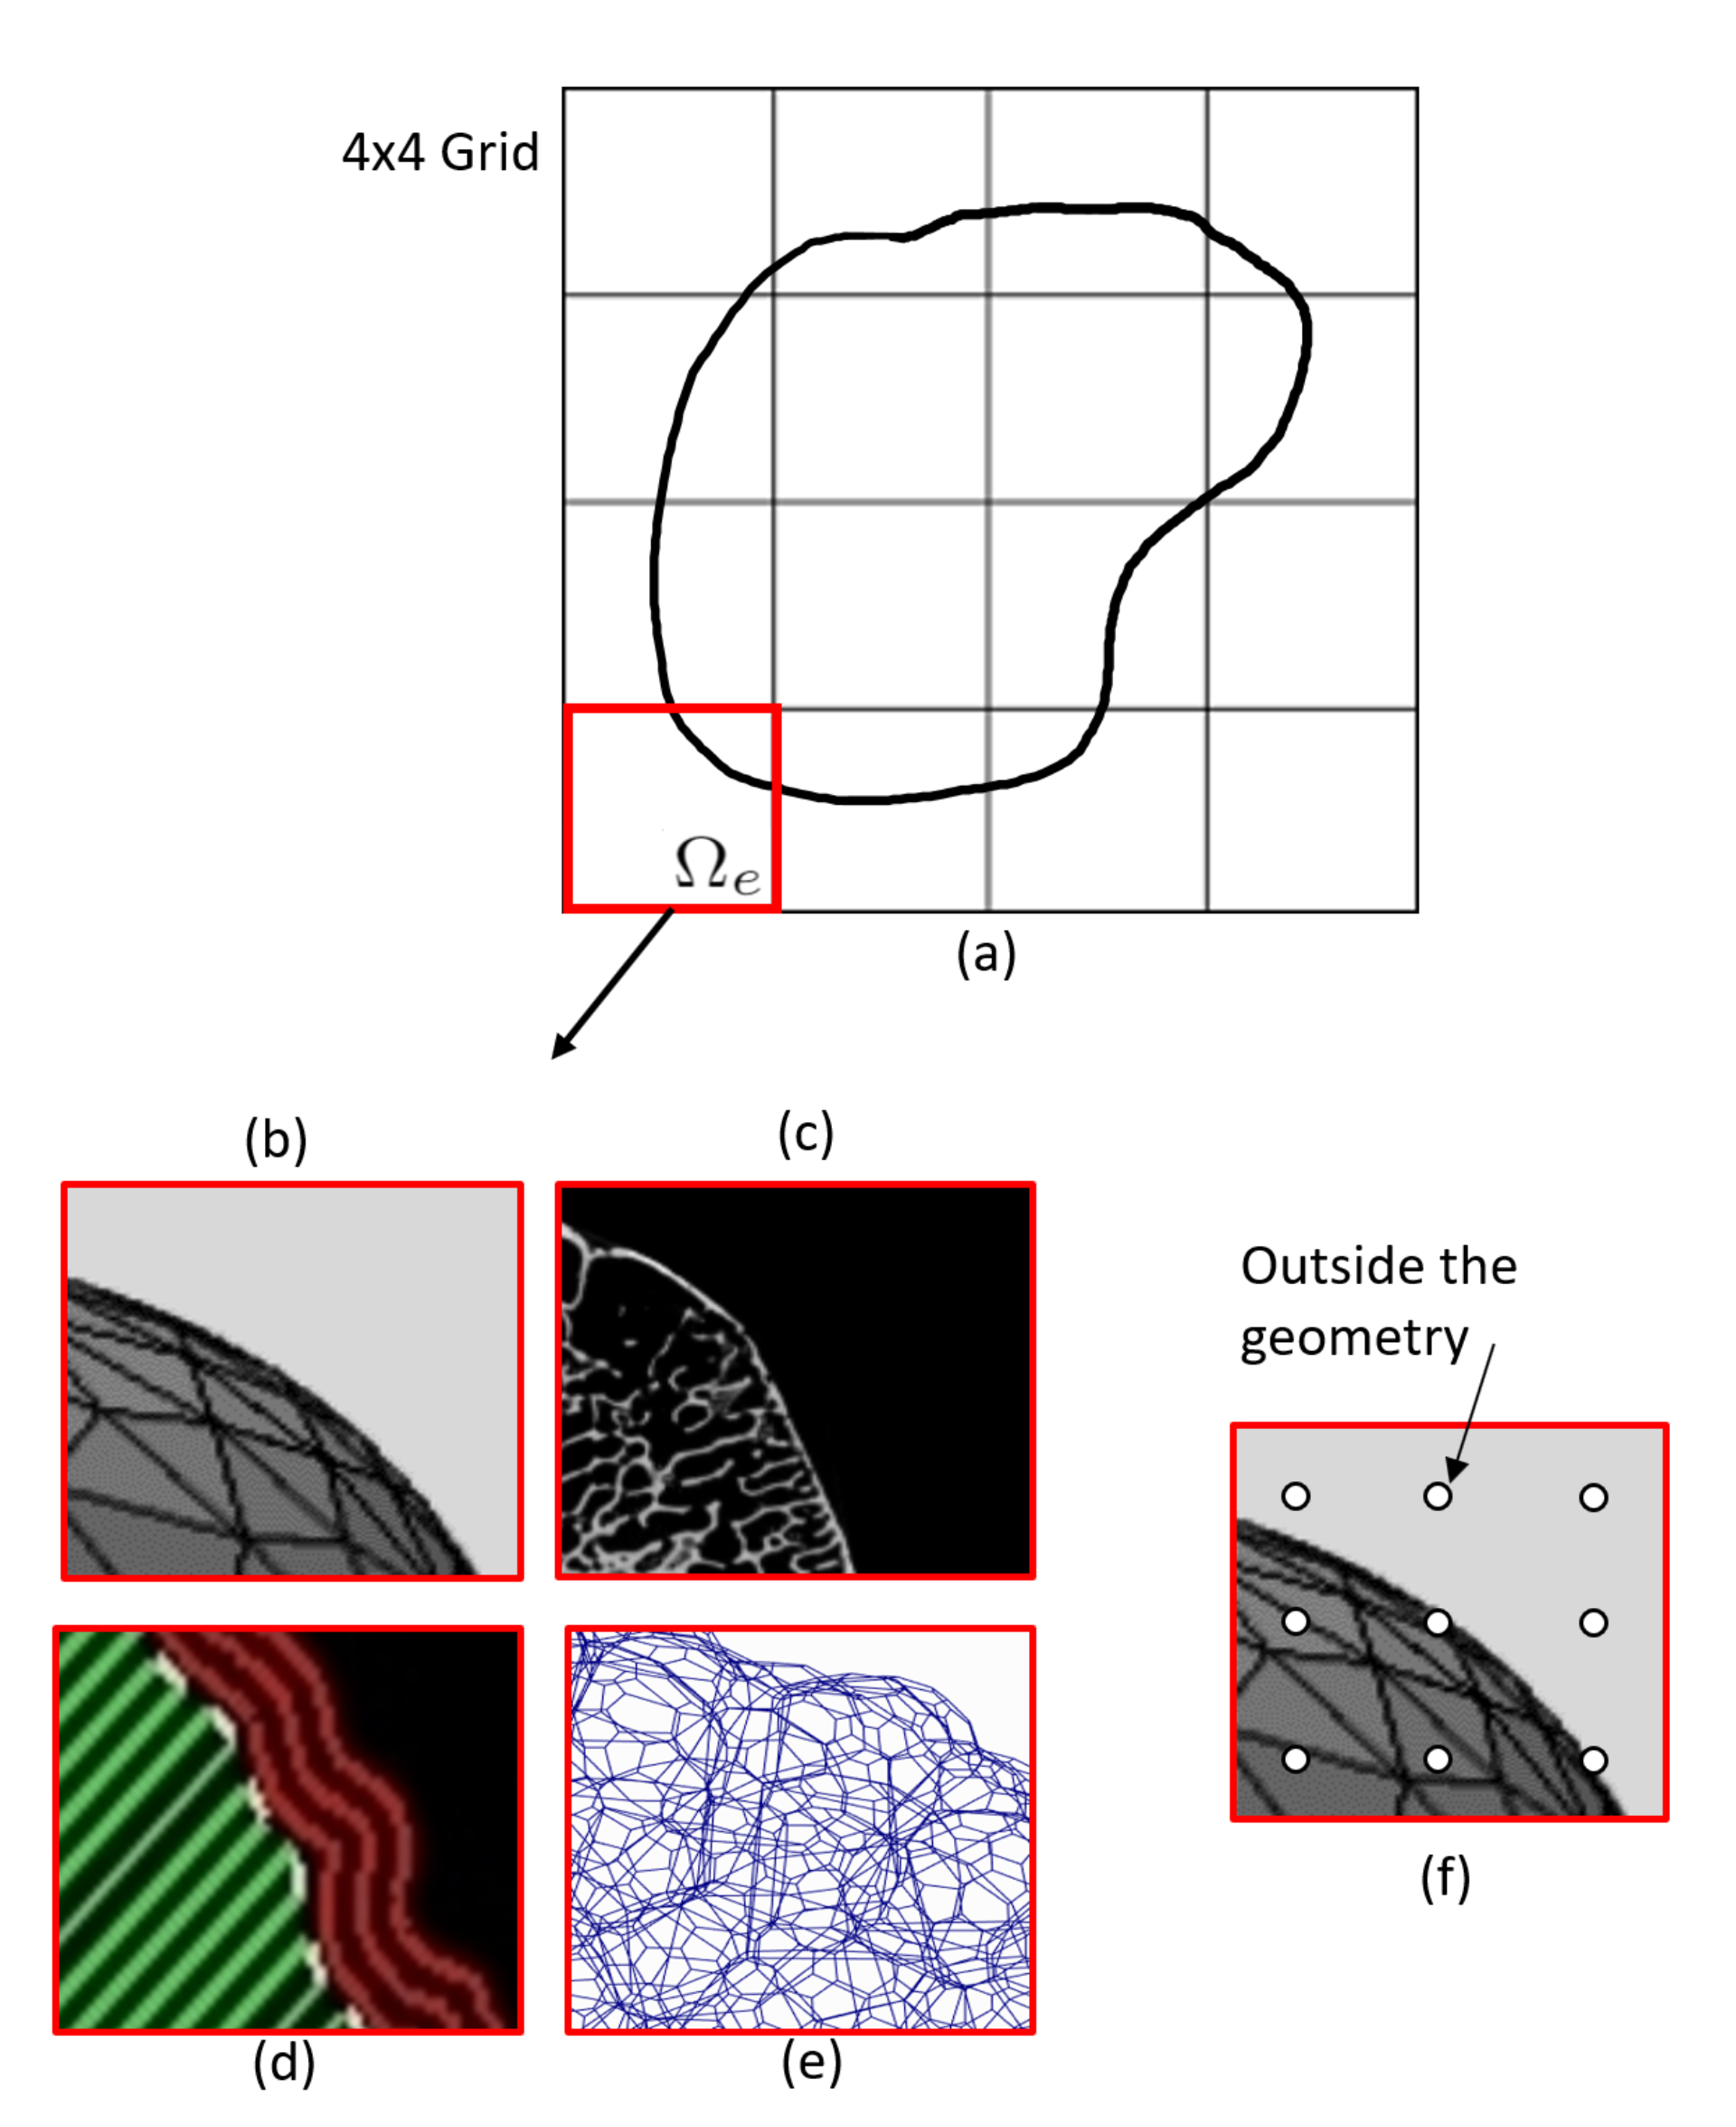
\includegraphics[width=4cm]{immersed_moments.png} 
\end{center}
\end{columns}
\blfootnote{Image from \cite{Taber2018}}
\end{frame}

\begin{frame}{Conclusion}
\begin{columns}
\column{0.58\linewidth}
\begin{center}
\begin{outline}
\1 Today we covered:
\2 Finite Element Analysis
\2 Quadrature Rules
\2 Moment Fitting
\1 Questions?
\end{outline}
\end{center}

\column{0.38\linewidth}
\begin{center}
\shadowimage[width=4cm]{thanks.jpg} 
\end{center}

\end{columns}
\end{frame}
